%%%%%%%%%%%%%%%%%%%%%%%%%%%%%%%%%%%%%%%%%
% University Assignment Title Page 
% LaTeX Template
% Version 1.0 (27/12/12)
%
% This template has been downloaded from:
% http://www.LaTeXTemplates.com
%
% Original author:
% WikiBooks (http://en.wikibooks.org/wiki/LaTeX/Title_Creation)
%
% License:
% CC BY-NC-SA 3.0 (http://creativecommons.org/licenses/by-nc-sa/3.0/)
% 
% Instructions for using this template:
% This title page is capable of being compiled as is. This is not useful for 
% including it in another document. To do this, you have two options: 
%
% 1) Copy/paste everything between \begin{document} and \end{document} 
% starting at \begin{titlepage} and paste this into another LaTeX file where you 
% want your title page.
% OR
% 2) Remove everything outside the \begin{titlepage} and \end{titlepage} and 
% move this file to the same directory as the LaTeX file you wish to add it to. 
% Then add \input{./title_page_1.tex} to your LaTeX file where you want your
% title page.
%
%%%%%%%%%%%%%%%%%%%%%%%%%%%%%%%%%%%%%%%%%
%\title{Title page with logo}
%----------------------------------------------------------------------------------------
%	PACKAGES AND OTHER DOCUMENT CONFIGURATIONS
%----------------------------------------------------------------------------------------

\documentclass[12pt]{article}
\usepackage[english]{babel}
\usepackage[utf8x]{inputenc}
\usepackage{amsmath}
\usepackage{graphicx}
\usepackage{listings}  
\usepackage[colorinlistoftodos]{todonotes}

\begin{document}

\begin{titlepage}

\newcommand{\HRule}{\rule{\linewidth}{0.5mm}} % Defines a new command for the horizontal lines, change thickness here

\center % Center everything on the page
 
%----------------------------------------------------------------------------------------
%	HEADING SECTIONS
%----------------------------------------------------------------------------------------

\textsc{\LARGE Memorial University of Newfoundland}\\[1.5cm] % Name of your university/college
\textsc{\Large CMSC6950}\\[0.5cm] % Major heading such as course name
\textsc{\large Group Project}\\[0.5cm] % Minor heading such as course title

%----------------------------------------------------------------------------------------
%	TITLE SECTION
%----------------------------------------------------------------------------------------

\HRule \\[0.4cm]
{ \huge \bfseries Growing Degree Days }\\[0.4cm] % Title of your document
\HRule \\[1.5cm]
 
%----------------------------------------------------------------------------------------
%	AUTHOR SECTION
%----------------------------------------------------------------------------------------

\begin{minipage}{0.4\textwidth}
\begin{flushleft} \large
\emph{Author:}\\
Augustine \textsc{U.O}\\ % Your name
Obi Nixon\textsc{E.}\\ % Your name
Gurpreet Singh\\ % Your name
Sivachandran Bharathi\\ % Your name
Adeoya Adebayo\\ % Your name
Boxuan Li % Your name
\end{flushleft}
\end{minipage}
~
\begin{minipage}{0.4\textwidth}
\begin{flushright} \large
\emph{Supervisor:} \\
Dr. Oliver Stueker\\ % Supervisor's Name
Shahrazad Malek\\ % Supervisor's Name
Prof. Ivan Saika-Voivod % Supervisor's Name
\end{flushright}
\end{minipage}\\[2cm]

% If you don't want a supervisor, uncomment the two lines below and remove the section above
%\Large \emph{Author:}\\
%John \textsc{Smith}\\[3cm] % Your name

%----------------------------------------------------------------------------------------
%	DATE SECTION
%----------------------------------------------------------------------------------------

{\large \today}\\[2cm] % Date, change the \today to a set date if you want to be precise

%----------------------------------------------------------------------------------------
%	LOGO SECTION
%----------------------------------------------------------------------------------------


 
%----------------------------------------------------------------------------------------




\vfill % Fill the rest of the page with whitespace

\end{titlepage}

\begin{abstract}
The Growing Degree Day, or GDD, is a heat index that can be used to predict when a crop will reach maturity. Each day’s GDD is calculated by subtracting a reference temperature, which varies with plant species, from the daily mean temperature.
The reference temperature for a given plant is the temperature below which its development slows or stops. For example, cool season plants, have a reference temperature of 40 degrees fahrenheit while warm season plants, have a reference temperature of 50 degrees fahrenheit.
The development of plants depends on the accumulation of heat and since cool season plants have a lower reference temperature, they accumulate GDDs faster than warm season plants.\\
From http://whyfiles.org 
\end{abstract}

\section{Introduction}

From wikipedia.org: Growing degree day(s) (GDD), are a measure of heat accumulation used by horticulturists, gardeners, and farmers to predict plant and animal development rates such as the date that a flower will bloom, an insect will emerge from dormancy, or a crop will reach maturity.\\

Growing degree days take aspects of local weather into account and allow gardeners to predict the plants pace toward maturity.\\

The base temperature is that temperature below which plant growth is zero. GDs are calculated each day as maximum temperature plus the minimum temperature divided by 2 (or the mean temperature), minus the base temperature. GDUs are accumulated by adding each day’s GDs contribution as the season progresses.


\section{List of Cities }
This are the list of cities we used for this project:
\begin{enumerate}
\item St. John's Newfoundland.
\item Ontario Toronto.
\item British Columbia.
\end{enumerate}
\label{sec:examples}

\subsection{Download daily historical temperature}
The aim of this section is to download the historical temperature of several cities from the climate.weather database of Canada. The code below extracts the weather informations for the Station Ids, which we will use for the subsequent tasks in this project.   

\begin{lstlisting}[language=Python]
def download(stationid, year):
    
    
    print("Data for station with id {} for year {}".format(stationid, year))
    
    
    File_name = "{}_{}_t.csv".format(stationid, year)  #file name for the CSV
    url = "http://climate.weather.gc.ca/climate_data/bulk_data_e.html?format=csv&stationID="+str(stationid)+"&Year="+str(year)+"&Month=8&Day=1&timeframe=2&submit=Download+Data"

    #downloading the file from the URL, and Saving into CSV file
    if(os.path.exists('../Data_csv/'+File_name)): #download only if the file not Exists
        print("File Exists")
    else:
        print("Downloading in progress ...")
        try:
            urllib.request.urlretrieve(url, '../Data_csv/'+File_name)
        except FileNotFoundError as fnfe:
            print("File not found..")
            print("%s" % fnfe)
            return ""
        except Exception as e:
            print("%s" % e)
            return ""
            
        print("Download Completed...")
        
\end{lstlisting}

\subsection{Annual Cycle of Min/Max Daily Temperatures Plots }
In this subsection, we used the downloaded data from the earlier task to create a 3 plots of the selected Canadian cities showing an annual cycle of the minimum or maximum daily temperatures. The min and max temperatures will be used when calculating the GDD in the next task. \\
When the min-max function is called, the download function gets the information from the station id and year supplied. From the database extracted, we get the min and max temperature  which will be used for the plots. 
Below are the min/max plots for our 3 selected cities:\\


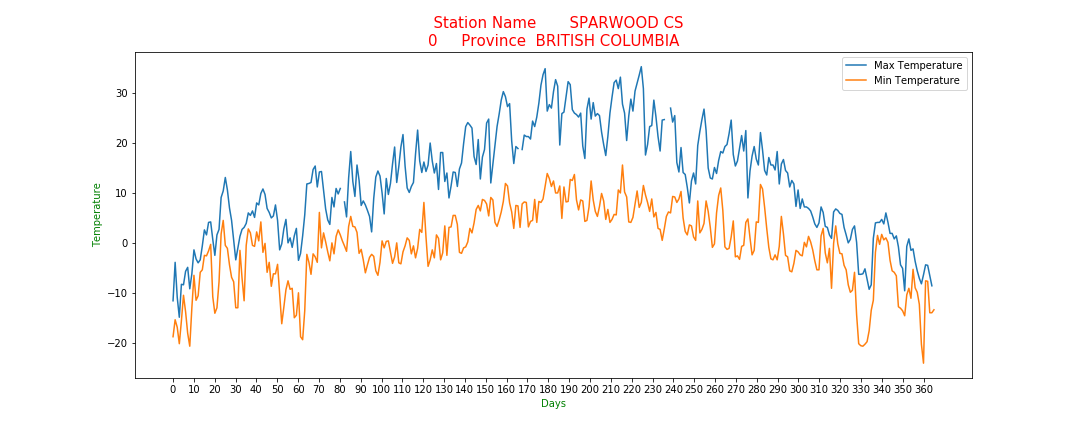
\includegraphics[scale=0.35]{Fig_6842_2015.png}\\

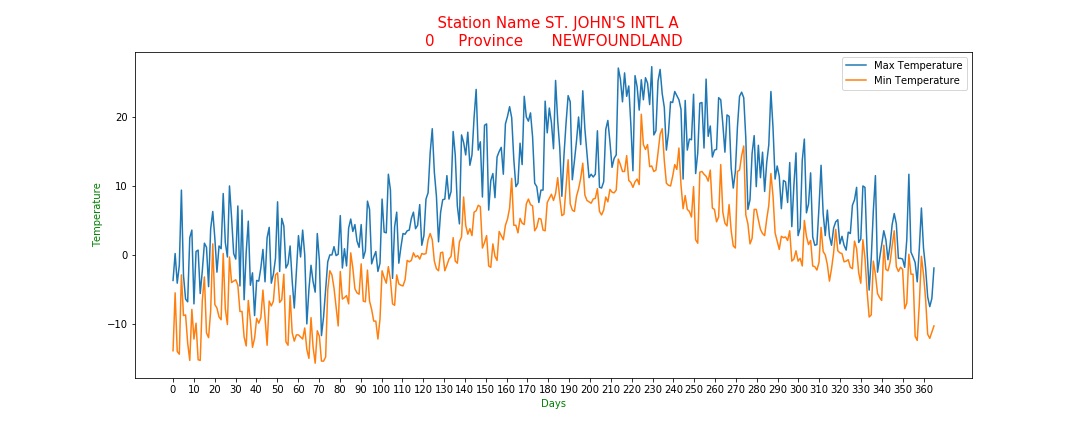
\includegraphics[scale=0.35]{Fig_50089_2015.png}\\

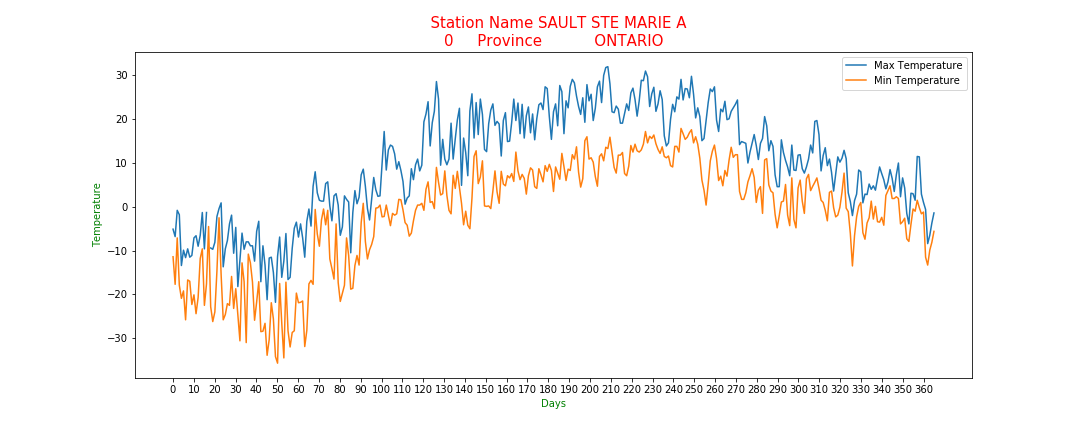
\includegraphics[scale=0.35]{Fig_50092_2015.png}\\

Plotting with Bokeh plot\\

\includegraphics[scale=0.35]{Screen_Shot_1.png}\\
\includegraphics[scale=0.35]{Screen_Shot_2.png}\\
\includegraphics[scale=0.35]{Screen_Shot_3.png}\\



\subsection{Calculating the GDD}

To calculate the GDD, we had to use maximum temperature plus the minimum temperature divided by 2 (or the mean temperature), minus the base temperature.\\
GDD are calculated by taking the integral of warmth above a base temperature, $T_{{\mathrm  {base}}} (usually 10 °C):$\\
GDD can be calculated using this formulae:

$$GDD={\frac  {T_{{\mathrm  {max}}}+T_{{\mathrm  {min}}}}{2}}-T_{{\mathrm  {base}}}. $$\

The code below is for calculating GDD:\\
--Note this is not all the code--\\

\begin{lstlisting}[language=Python]
import numpy as np
import download_data as DW
import math

def gdd_tot(mean):
     temp = 0.0
     for i in mean:
         if i < 10.0:
             temp = temp + 0.0
         elif not math.isnan(i) :
             temp = temp + (i - 10.0)
     return temp

\end{lstlisting}

With the gdd-total function, we created a function gdd-cal which will calculate the accumulated gdd for each month using the gdd-total and the gdd-accum will calculate the total of of all the months  .\\
The data calculated will be used to plot the graphs in the next task.
  
\subsection{Plots Showing Accumulated GDD vs Time for\\ Selected Cities}

Here we use the results from our calculation above to create plots showing the accumulate GDD vs Time for selected cities. 

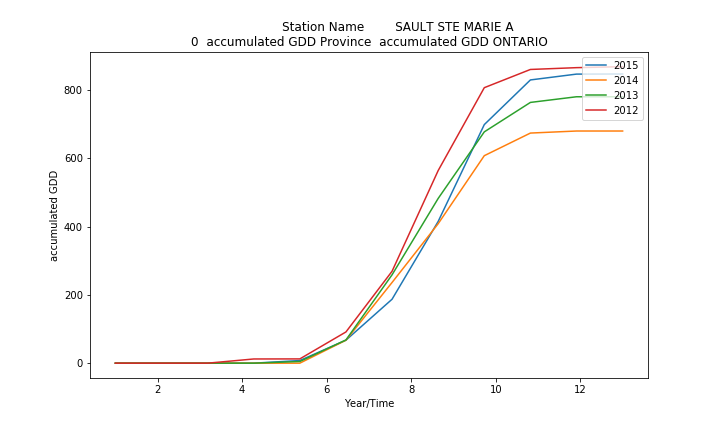
\includegraphics[scale=0.35]{Fig_GDD_50092.png}\\

Bokeh Plots:\\

\includegraphics[scale=0.35]{Screen_Shot_4.png}\\
\includegraphics[scale=0.35]{Screen_Shot_5.png}\\
\includegraphics[scale=0.35]{Screen_Shot_6.png}\\
\includegraphics[scale=0.35]{Screen_Shot_7.png}\\
  

\subsection{Secondary Tasks}
The plots below for showing GDD:\\

\includegraphics[scale=0.35]{Screen_Shot_8.png}\\
\includegraphics[scale=0.35]{Screen_Shot_9.png}\\
\includegraphics[scale=0.35]{Screen_Shot_10.png}\\
\includegraphics[scale=0.35]{Screen_Shot_11.png}\\

Exploring how GDD calculations depends on the choice of Tbase:\\

\includegraphics[scale=0.35]{Screen_Shot_12.png}\\
\includegraphics[scale=0.35]{Screen_Shot_13.png}\\
\includegraphics[scale=0.35]{Screen_Shot_14.png}\\
\includegraphics[scale=0.35]{Screen_Shot_15.png}\\





\end{document}
